\documentclass[12pt]{report}
\usepackage{titlesec}
\usepackage[dvips]{graphicx}
\usepackage[below]{placeins}
\usepackage[margin=1.2in]{geometry}
\usepackage{amssymb}
\usepackage{url}
\usepackage{fancyhdr}

\setlength{\parindent}{0pt}
\setlength{\parskip}{0.60\baselineskip}
\setlength{\marginparwidth}{1in}

\begin{document}

\newcommand{\btr}{\-$\blacktriangleright$\-}

\newcommand{\mybox}[1]{\vspace{5pt}%
\begin{center}\begin{tabular}{|p{0.75\textwidth}|}\hline\vspace{1pt}\hfill\ttfamily #1 \hfill\vspace{7pt}\\ \hline %
\end{tabular}\end{center}\vspace{5pt}}

\titleformat{\chapter}[display]
{\normalfont\large\sffamily}
{\titlerule[0.5pt]%
 \vspace{2pt}
 \titlerule[1pt]%
 \vspace{2pt}%
 \titlerule[2pt]%
 \vspace{2pt}%
 \titlerule[1pt]%
 \vspace{1pc}\large CHAPTER \thechapter}
{1pc}
{\Huge}[\vspace{10pt}\titlerule]

\titleformat{\section}[block]
 {\normalfont\sffamily}
 {\Large\bfseries\thesection}{.5em}{\Large\bfseries}

\titleformat{\subsection}[block]
 {\normalfont\sffamily}
 {\large\bfseries\thesubsection}{.5em}{\large\bfseries}

%%%% cover
\newpage
\pagestyle{empty}

{\Large\sffamily\bfseries SpineSeg -- \mdseries Semi-Automatic Spinal Cord Segmentation}

{\Large Usage Guide}

\vspace{1in}

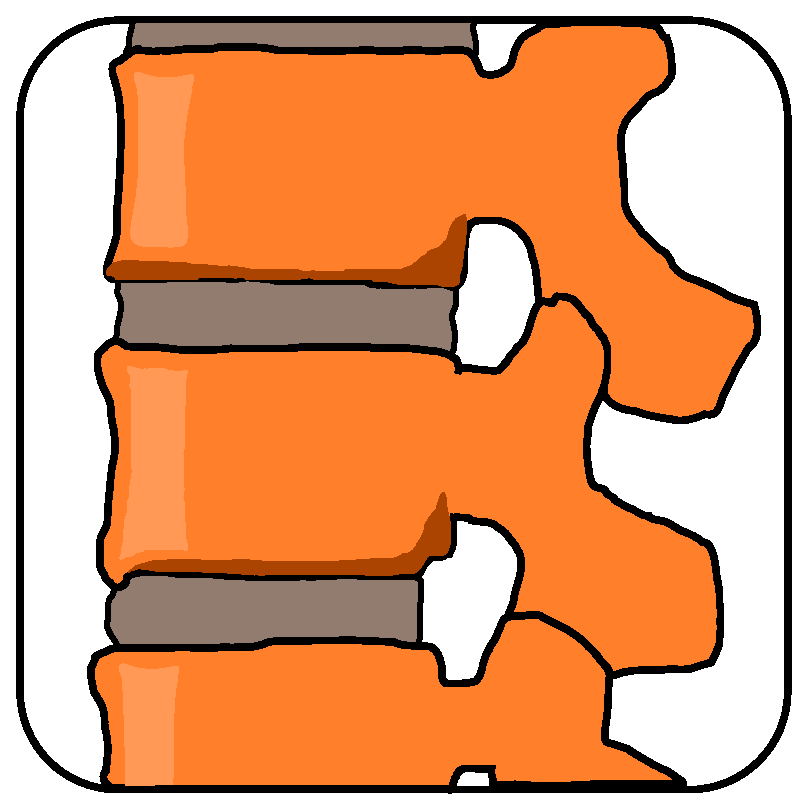
\includegraphics[height=4in]{logo.eps}

\vspace{1in}

{\large\sffamily February 2011 (Version 2.0)} 

{\Large\sffamily\bfseries Felipe P. G. Bergo} 

%%%% face page
\newpage
\pagestyle{empty}

{\Large\sffamily\bfseries SpineSeg -- \mdseries Semi-Automatic Spinal Cord Segmentation}

{\Large Usage Guide}

\vspace{3cm}

\copyright 2011 Felipe P. G. Bergo\\

\texttt{felipe@bergo.eng.br} \\

\vspace{1cm}

This guide is available for free download at \\
\url{http://www.liv.ic.unicamp.br/~bergo/spineseg}. \\ 
Sale of this manual, in either electronic or printed form, is forbidden.

\vspace{3cm}

Version History: \\

\begin{tabular}{|l|p{3.5in}|}
\hline
2011.02.03 & first version of the guide, written for SpineSeg 2.0. \\
\hline
\end{tabular}

%%% 
\newpage
\tableofcontents
\pagestyle{fancy}
\lhead{\sffamily\bfseries SpineSeg \rmfamily\mdseries Usage Guide}
\chead{}
\rhead{}
\lfoot{}
\cfoot{\thepage}
\rfoot{}
\renewcommand{\headrulewidth}{0.4pt}
\renewcommand{\footrulewidth}{0.4pt}

%%%
\chapter{Installation}
\label{c.install}

\section{Introduction}

SpineSeg is a medical image analysis tool developed to evaluate spinal
cord atrophy in MR volumes. It is distributed with source code under
the terms of the GNU General Public License, version 2. SpineSeg is
based on the GTK+ toolkit and works on Unix-like systems such as
Linux, FreeBSD and Mac OS X.

\section{SpineSeg Installation}

SpineSeg is distributed in source code form and its compilation
requires a working set of Unix-compatible development utilities, the
GNU C++ compiler and the GTK+ toolkit with development headers
installed, version 2.6.0 or later. These are easily found on most
current Linux operating system distributions.

The SpineSeg source code package can be downloaded from
\url{http://www.liv.ic.unicamp.br/~bergo/spineseg}, and the following
commands can be used to unpack, compile and install it:

\begin{verbatim}
tar zxvf spineseg-2.0.tar.gz
cd spineseg-2.0
./configure
make
make install
\end{verbatim}

By default, the install prefix will be set to \texttt{/usr/local}. The
user running the last step (make install) must have write permission
to the installation prefix. The installation prefix can be customized
with

\mybox{./configure --prefix=/custom/path}

SpineSeg uses the GNU autotools for package configuration, and further
customization options can be listed with

\mybox{./configure --help}

With the default prefix, the spineseg program executable will with
installed in \texttt{/usr/local/bin}, icons will be installed in
\texttt{/usr/local/share/pixmaps}, documentation and sample MR data in
\texttt{/usr/local/share/spineseg}.

SpineSeg is known to work in the following operating systems and distributions:

\begin{itemize}
\item Fedora Linux (tested with versions 12, 13 and 14).
\item Ubuntu Linux (tested with version 10.10)
\item CentOS Linux (tested with versions 4.4, 5.1, 5.2, 5.3)
\item FreeBSD 6.1
\item Mac OS X (tested with version 10.6 (Snow Leopard))
\end{itemize}

\section{Image Conversion Utilities}

To convert images from standard formats such as DICOM and Analyze to SpineSeg's SCN, 
users will want dicom2scn, IVS and/or Aftervoxel. \textbf{dicom2scn} is an
open source command-line utility for format conversion, it converts
DICOM to SCN and also includes utilities to convert between SCN and
the popular Analyze format. dicom2scn can be downloaded from

\mybox{\url{http://www.liv.ic.unicamp.br/~bergo/ivs}}

and compiled and installed with 

\begin{verbatim}
tar zxvf dicom2scn-2010.2.tar.gz
cd dicom2scn-2010.2
make
make install
\end{verbatim}

The dicom2scn installation prefix is defined as \texttt{/usr/local} in
the Makefile. To change it, edit the Makefile.

IVS and Aftervoxel are graphical medical image processing applications
for Linux, distributed as freeware (no source code available). IVS can
read/write SCN and Analyze formats, and includes dicom2scn as a
command-line tool. Aftervoxel can read DICOM, SCN and Analyze, and write SCN
and Analyze. Aftervoxel provides a graphical interface for DICOM importing,
and may be desirable for users not used to command-line utilities. IVS and
Aftervoxel can be downloaded from the addresses below:

\mybox{\url{http://www.liv.ic.unicamp.br/~bergo/ivs}}

\mybox{\url{http://www.liv.ic.unicamp.br/~bergo/aftervoxel}}

\chapter{User Interface}
\label{c.ui}

\section{Running SpineSeg}

SpineSeg can be started with

\mybox{spineseg \&}

Started with no parameters, it will interpolate axial slices to 0.50 mm. The
following command-line options can be used:

\begin{description}
\item[-debug] Enable debugging actions. In the current version, it will save intermediary
segmentation results to SCN files in the current working directory.
\item[-r value] Overrides the axial interpolation resolution to the given value in
millimeters.
\item[-c] Enable axial slice compositing. With compositing enabled,
  each slice is averaged from the nearest 3 slices, effectively
  multiplying thickness by 3.
\item[-g value] Overrides the morphological gradient radius used for tree pruning preprocessing.
The default is a 1.0-pixel radius. Larger radii increase the gradient border barriers
for tree-pruning, reducing leaking.
\item[-h] Shows a summary of command-line options on the standard output and exits.
\end{description}

\section{Loading Volumes}

SpineSeg can only read volumes in the SCN format (created at the
Institute of Computing, Unicamp).  Volumes can be loaded with the
\emph{File \btr Load Volume} and \emph{File \btr Load Special}
commands.  The first one requires that volume files be in sagittal
orientation, with the Z coordinate increasing from left to right. The
second command allows the user to choose orientation, as well as
override slice compositing and axial resolution interpolation (Figure~\ref{f.loadspecial}).

\begin{figure}[!htb]
\begin{center}
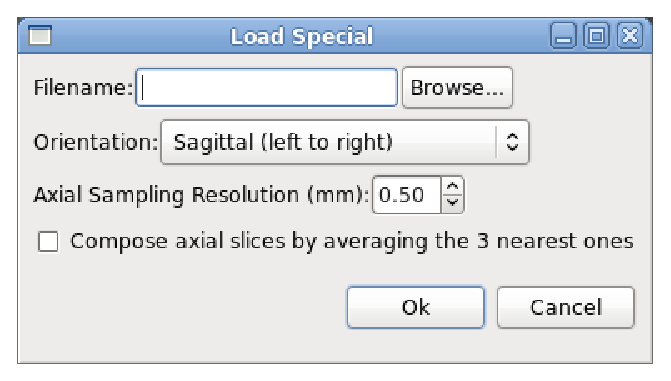
\includegraphics[width=8cm]{loadspecial.eps}
\caption{Load Special dialog.}
\label{f.loadspecial}
\end{center}
\end{figure}

\section{Tools}

Once a volume has been loaded, the main window will appear as
illustrated in Figure~\ref{f.main}.  The left pane displays either a
sagittal or coronal view, and the right pane displays an axial
view. The six buttons on the top left allow the user to switch between
tool modes (Zoom, Pan, Reslice, Semi-automatic segmentation, Manual
Segmentation and Distance Measurement, respectively).  The Window,
Opacity, Show PIP and Show fit controls on the bottom right control
the viewing parameters.

\begin{figure}[!htb]
\begin{center}
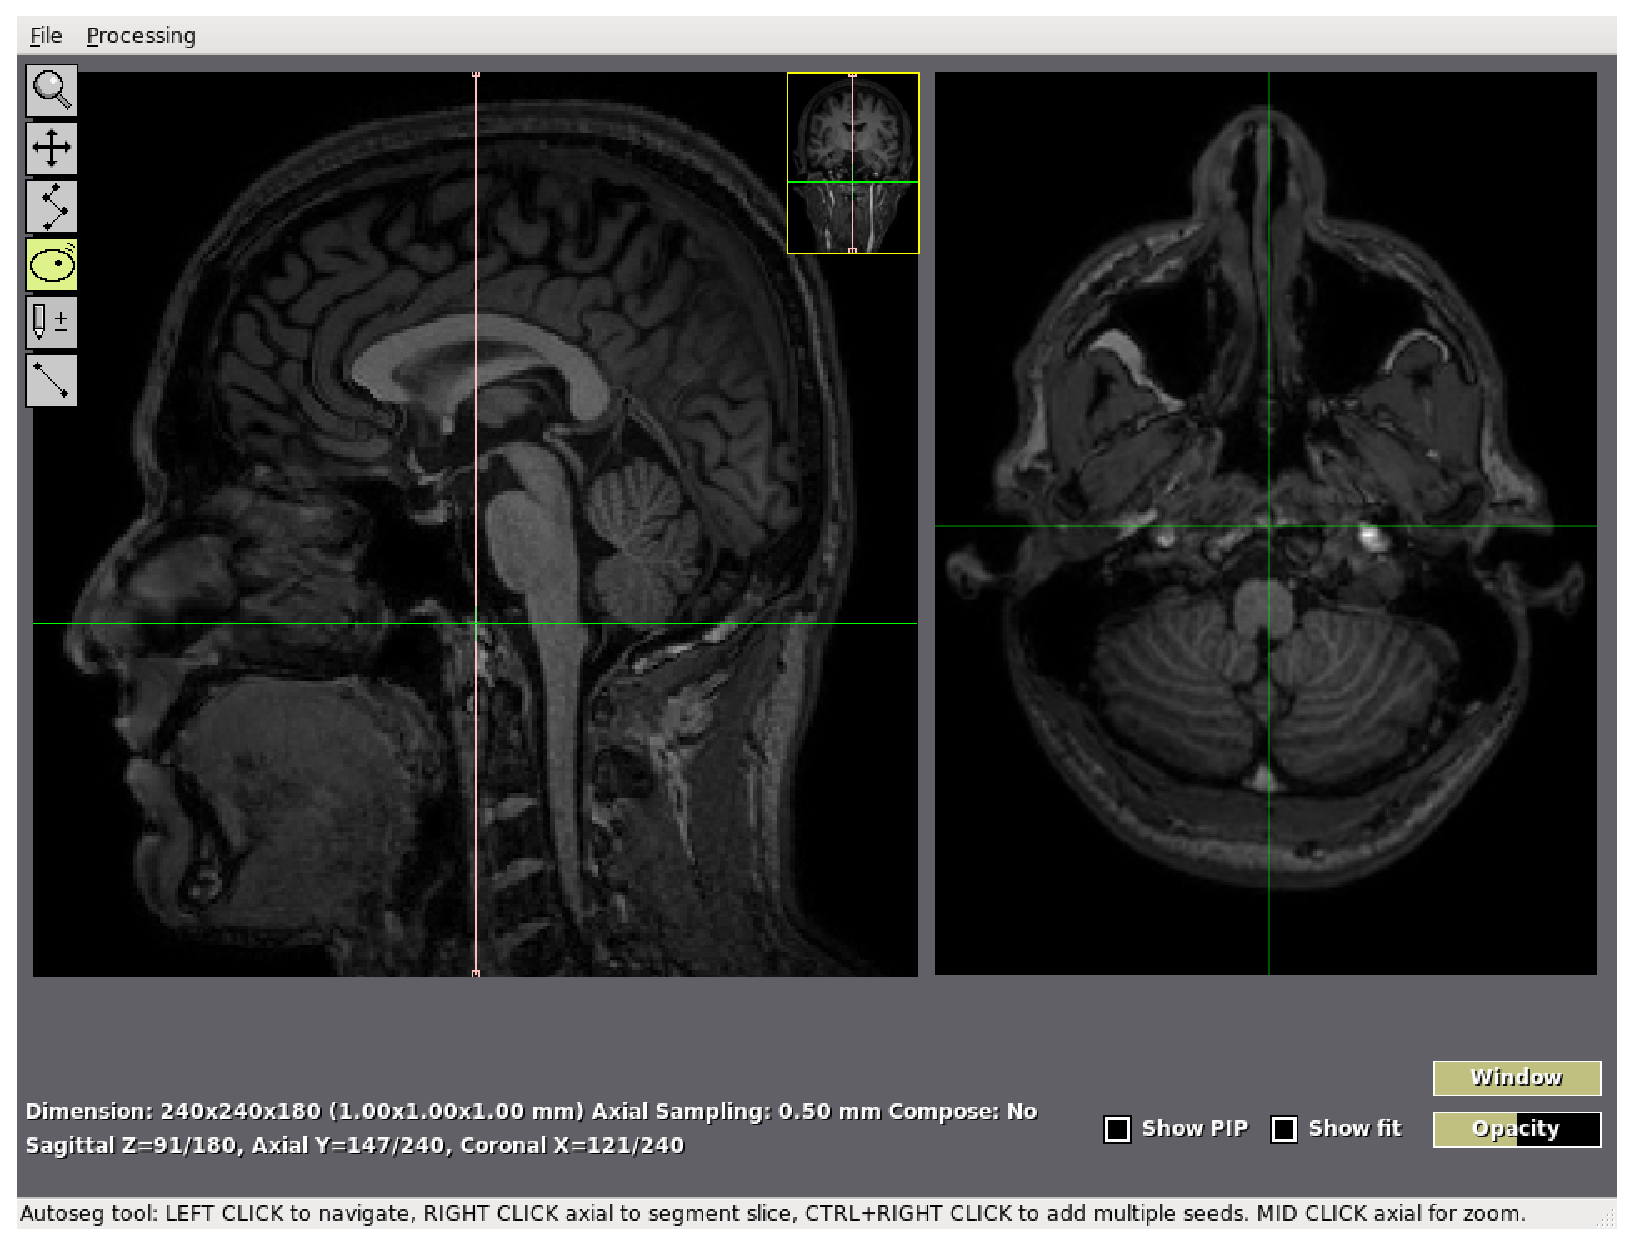
\includegraphics[width=0.90\textwidth]{main.eps}
\caption{Main window after loading a volume.}
\label{f.main}
\end{center}
\end{figure}

\subsection{Sagittal/Coronal Alternation}

When ``Show PIP'' checkbox is activated, a small window with a
sagittal or coronal slice is shown on the top right corner of the left
image pane. Clicking on the small preview will switch between Sagittal
and Coronal views.

\subsection{Window Control}

The ``Window'' control on the bottom right of the main window controls
the visualization brightness. In the default (maximum) setting, the
highest voxel intensity is displayed as white. Reducing the window
level lowers the white saturation point, enhancing brightness and
contrast of the the displayed image. This control only affects
visualization and has no effect on any image processing algorithm
within SpineSeg.

\subsection{Right Pane Zoom}

An additional zoom level of 2X, 4X or 8X can be set for the right
pane. The zoom modes can be switched by clicking the right pane with
the middle mouse button, or with the 'Z' key on the keyboard. When the
right pane zoom is set to anything but 1X, the zoom level is shown
between square brackets on the right pane.

\subsection{Zoom Tool}

When the Zoom tool is activated, clicking with the left mouse button
anywhere on the screen will control the overall zoom level. A zoom
level bar will be displayed and can be controlled by dragging the
mouse horizontally. To reset the zoom level to fit the window, click
anywhere with the right mouse button while this tool is selected.

\subsection{Pan Tool}

When the Pan tool is activated, dragging the mouse with the left
button pressed will pan (translate) the entire view within the
window. To reset the pan state, click anywhere with the right mouse
button while this tool is selected.

\subsection{Reslice Tool}

The reslice tool allows the user to edit the guiding curves (pink
lines on the left pane) on the sagittal and coronal views and
regenerate the axial slices such that they are orthogonal to
them. When the reslice tool is selected, two buttons are shown near
the tool button. ``Linear/Spline'' indicates the curve interpolation
mode, and can be clicked to alternate between them
(Figure~\ref{f.reslice}). ``Reslice'' interpolates all axial slices to
fit the current guiding curves. When the curves have been edited, and
the axial view is invalid, the right pane will be tonalized in
red. Clicking with the left mouse button on the left pane adds a
control point to the guide curve, and clicking with the right mouse
button (on the left pane) deletes the nearest control
point. Left-clicking the right pane moves the cursor, allowing the
user to view different slices on the left pane.

\begin{figure}[!htb]
\begin{center}
\begin{tabular}{cc}
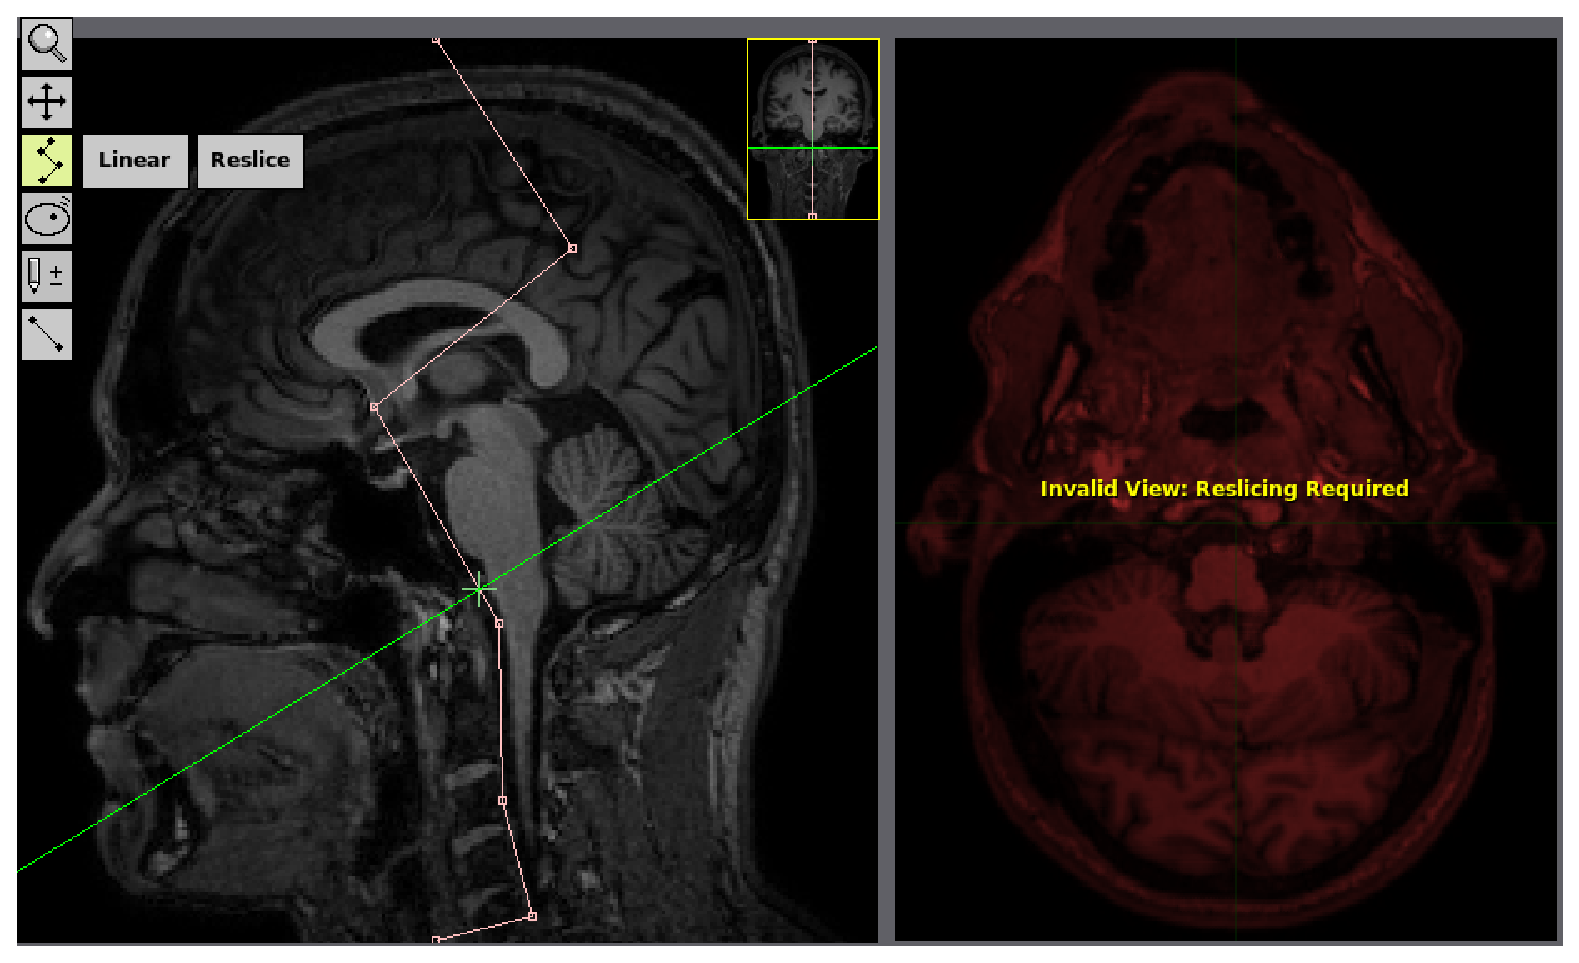
\includegraphics[width=.47\textwidth]{reslice1.eps} & %
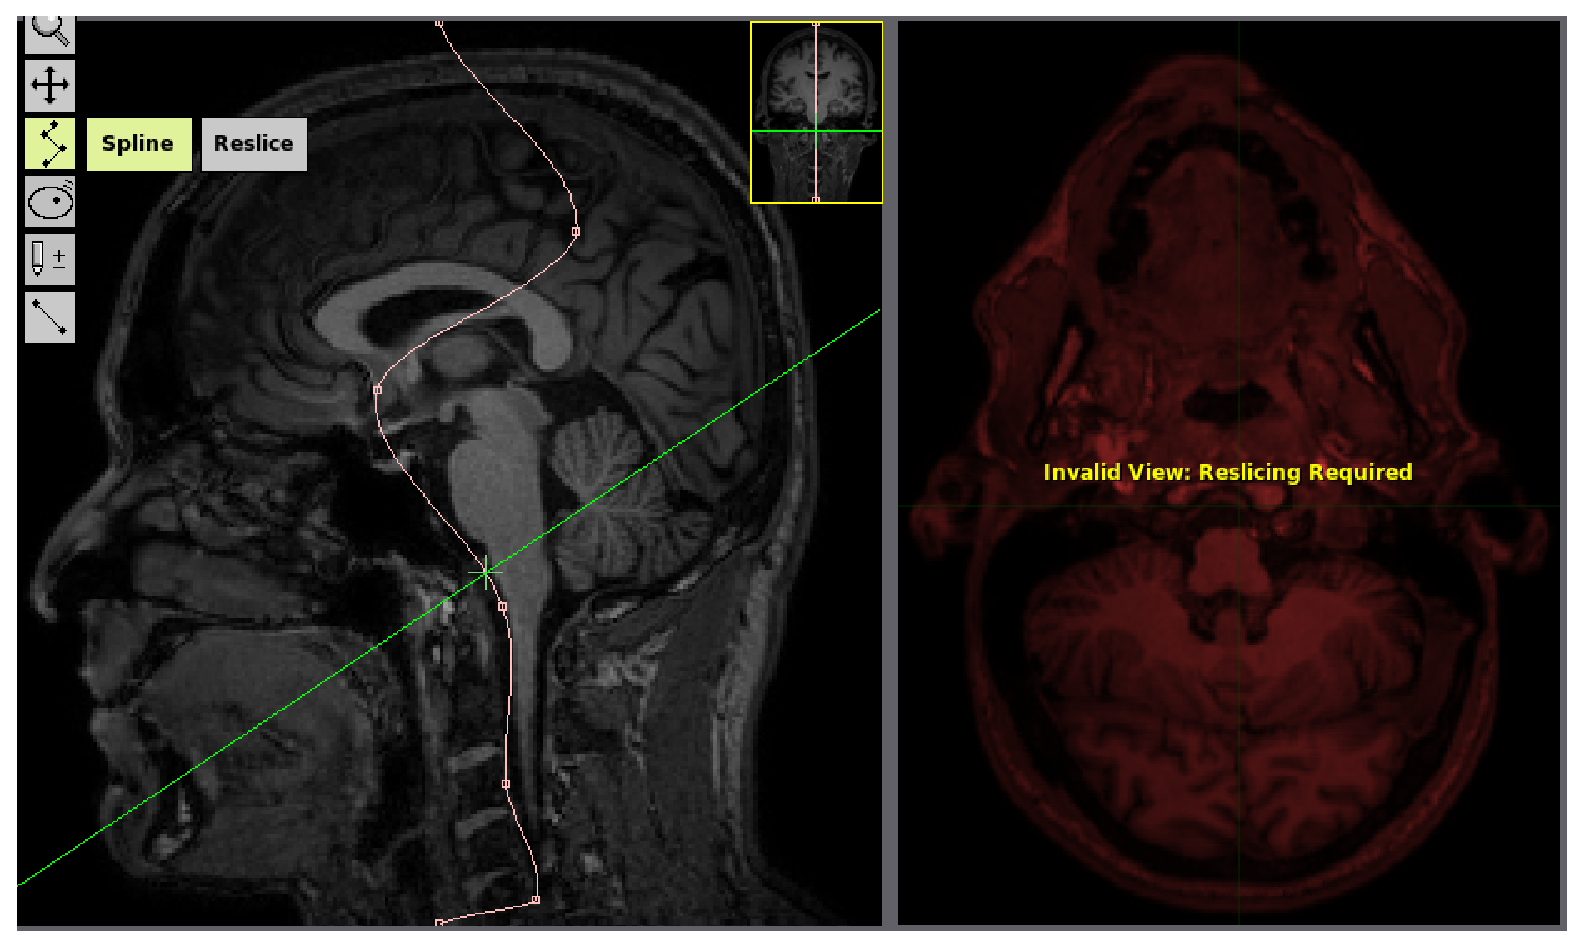
\includegraphics[width=.47\textwidth]{reslice2.eps} \\ 
(a) & (b)
\end{tabular}
\caption{Reslice Tool: (a) Linear interpolation. (b) Spline interpolation.}
\label{f.reslice}
\end{center}\end{figure}

\subsection{Semi-Automatic Segmentation Tool}

When this tool is selected, clicking on any image pane with the left
mouse button moves the cursor, changing the current slice. Clicking on
the right pane with the right button performs tree-pruning
segmentation on that slice with a single seed at the point clicked. To
add more seeds, click with the right button while holding the
\emph{Ctrl} key. Seeds are shown as red pixels.  Once an object has
been segmented, it is tonalized in yellow on the right pane, its
ellipse fitting is drawn in cyan. The opacity of the object
tonalization can be changed at the ``Opacity'' control on the bottom
right. The display of the ellipse fit can be toggled with the ``Show
fit'' checkbox. An orange marker is shown on the left pane for each
slice where some segmentation has been performed. The segmentation
measurements and fitted ellipse properties are shown on the third line
of text below the image panes. Figure~\ref{f.auto} illustrates a slice
with semi-automatic segmentation performed.

\begin{figure}[!htb]
\begin{center}
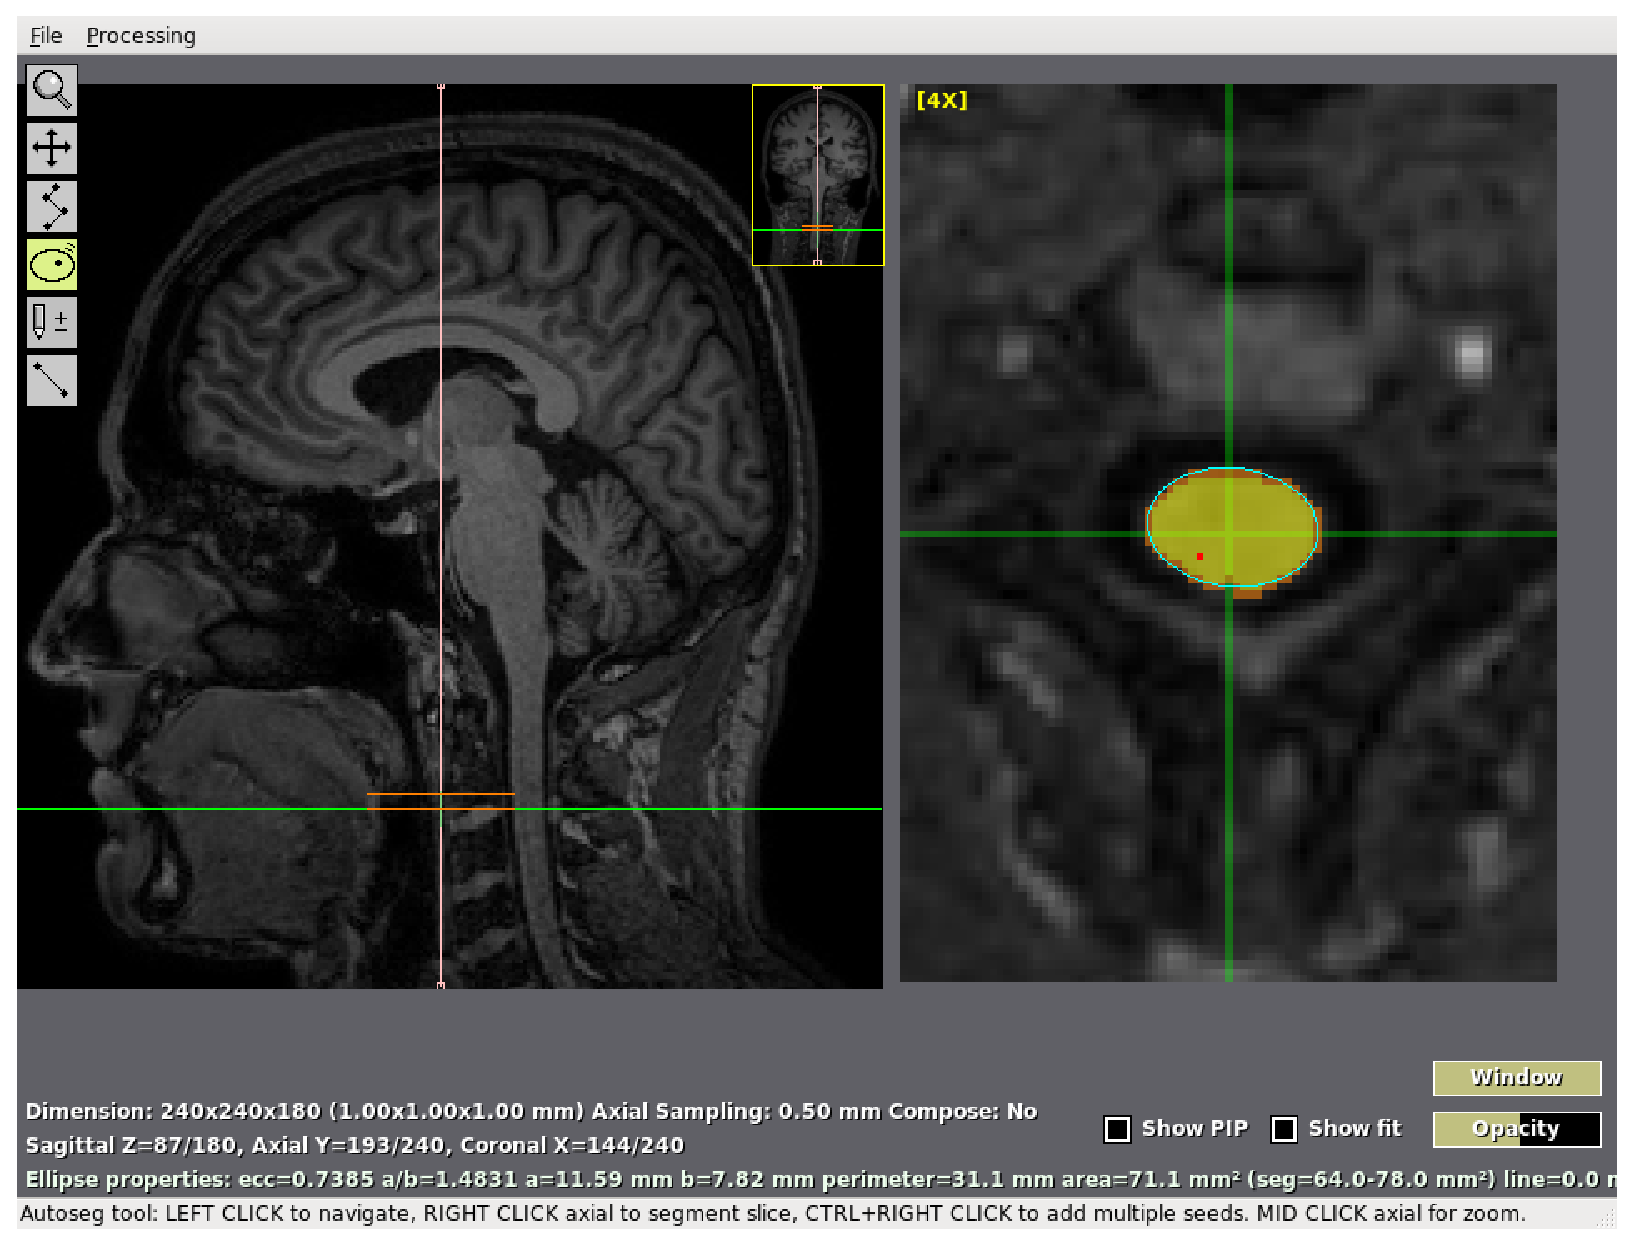
\includegraphics[width=0.65\textwidth]{auto.eps}
\caption{Interface showing a slice with semi-automatic segmentation.}
\label{f.auto}
\end{center}
\end{figure}

\subsection{Manual Segmentation Tool}

When this tool is selected, clicking on the right pane adds (left
button) or removes (right button) border points. When at least 6
points are present on a slice, an ellipse is fitted to
them. Figure~\ref{f.manual} shows an ellipse fitted to manual border
points. Clicking on the left pane moves the cursor and changes the
slice currently displayed.

\begin{figure}[!htb]
\begin{center}
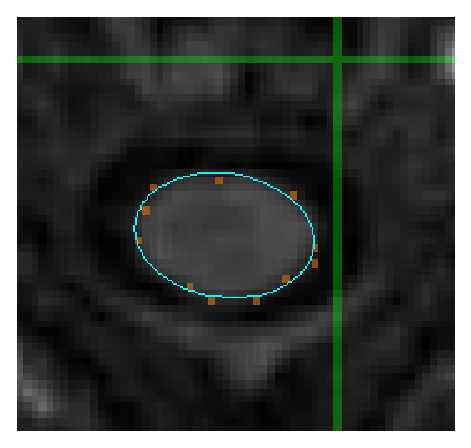
\includegraphics[width=5cm]{manual.eps}
\caption{Ellipse fitted to manually-added border points.}
\label{f.manual}
\end{center}
\end{figure}

\subsection{Distance Measurement Tool}

When this tool is selected, clicking on the right pane sets the
endpoints of a ruler (show in magenta, Figure~\ref{f.ruler}). SpineSeg
supports only one distance measurement per slice, and the distance
measured is shown on the third text line below the image panes.
Clicking on the right pane when a ruler is already set moves the
nearest endpoint to the clicked location.  Clicking on the left pane
moves the cursor and changes the slice currently displayed.

\begin{figure}[!htb]
\begin{center}
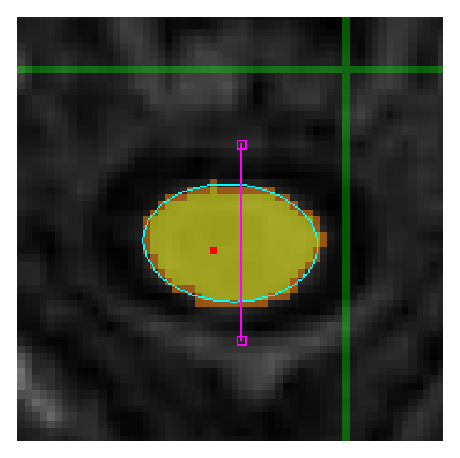
\includegraphics[width=5cm]{ruler.eps}
\caption{Distance measurement (Ruler).}
\label{f.ruler}
\end{center}
\end{figure}

\newpage
\section{Keyboard Controls}

SpineSeg provides several keyboard shortcuts, which are independent of the
current tool selection:

\begin{center}
\begin{tabular}{|l|p{12cm}|}
\hline
Key & Action \\
\hline
F1 & Select the Zoom tool. \\
F2 & Select the Pan tool. \\
F3 & Select the Reslice tool. \\
F4 & Select the Semi-automatic segmentation tool. \\
F5 & Select the Manual segmentation tool. \\
F6 & Select the Distance measurement tool. \\
Del & Clear segmentations and measurements on the current slice. \\
Esc & Clear segmentations and measurements on the entire volume. \\
Arrow Keys & Move the cursor (up and down move along axial slices, left and right
move perpendicularly, depending on the sagittal/coronal state of the left pane). \\
F   & Toggle Show fit. \\
L   & Load volume. \\
S   & Alternate opacity between 0\% and 50\%. \\
Z   & Alternate between right pane zoom modes (1X, 2X, 4X, 8X). \\
-/+ & Control the Window setting. \\
9/0 & Control the Opacity setting. \\
\hline

\end{tabular}
\end{center}

\newpage
\section{Mouse Controls Summary}

The tables below summarize the action of each mouse button on each pane
according to the current tool. 

\subsection{Left Pane}

\begin{center}
\begin{tabular}{|l|l|l|l|}
\hline
Tool & Left & Middle & Right \\ %
\hline
\includegraphics[width=14pt]{zoom0.eps}   & Overall zoom & Right-pane zoom & Reset overall zoom  \\
\includegraphics[width=14pt]{pan0.eps}    & Pan          & Right-pane zoom & Reset pan \\
\includegraphics[width=14pt]{normal0.eps} & Add control point & Right-pane zoom & Remove control point \\
\includegraphics[width=14pt]{auto0.eps}   & Navigate     & Right-pane zoom &  \\
\includegraphics[width=14pt]{manual0.eps} & Navigate     & Right-pane zoom &  \\
\includegraphics[width=14pt]{dist0.eps}   & Navigate     & Right-pane zoom &  \\
\hline
\end{tabular}
\end{center}

\subsection{Right Pane}

\begin{center}
\begin{tabular}{|l|l|l|l|}
\hline
Tool & Left & Middle & Right \\ %
\hline
\includegraphics[width=14pt]{zoom0.eps}   & Overall zoom & Right-pane zoom & Reset overall zoom  \\
\includegraphics[width=14pt]{pan0.eps}    & Pan          & Right-pane zoom & Reset pan \\
\includegraphics[width=14pt]{normal0.eps} & Navigate     & Right-pane zoom & \\
\includegraphics[width=14pt]{auto0.eps}   & Navigate     & Right-pane zoom & Segment \\
\includegraphics[width=14pt]{manual0.eps} & Add point    & Right-pane zoom & Remove point \\
\includegraphics[width=14pt]{dist0.eps}   & Add endpoint & Right-pane zoom &  \\
\hline
\end{tabular}
\end{center}



\section{The Processing Menu}

The \emph{Processing} menu provides two image processing filters,
\emph{Gaussian Blur} and \emph{Median Filter} that can be used to smooth
noisy images. The Gaussian blur filters each axial slice with the kernel

\[
\left[
\begin{array}{ccc}
1 & 2 & 1 \\
2 & 4 & 2 \\
1 & 2 & 1
\end{array}
\right]
\]

The median filter processes each axial slice setting each pixel's intensity to the median
with the $3 \times 3$ block centered on it.

The processing menu also provides the \emph{Clear Volume} and \emph{Clear
  Slice} commands, that remove segmentations and rulers from the
entire volume and from the current slice, respectively.

\section{Saved States}

The state of a volume can be saved with the \emph{File \btr Save state} command. This command
saves all segmentations, reslicing state, and interface settings. The user must
have writing permissions to the directory where the volume was originally loaded from. 
Save states are automatically loaded by the \emph{Load Volume} and \emph{Load Special} commands.

The \emph{File \btr Clear Saved State} deletes the state files related to the current
volume, if they exist.

Naming and format of the state files are discussed in Chapter~\ref{c.savestate}.

\chapter{Usage Example}

In this chapter we show the typical procedure to measure the spinal
cord area using SpineSeg.  The axial resolution is study-dependent and
should be chosen in advance. For this example, we choose 0.60 mm. To
convert an image retrieved from the MR scanner in DICOM format, you
can use \emph{dicom2scn} utility described in
Chapter~\ref{c.install}. To convert a file named \texttt{IM1000.DCM}
located in the current directory with \emph{dicom2scn}, do:

\mybox{dicom2scn IM1000.DCM example.scn}

To run SpineSeg with the chosen resolution set, type in a terminal:

\mybox{spineseg -r 0.60 \&}

After the main window is shown, select \emph{File \btr Load Volume}
and pick the file \texttt{example.scn} converted on the previous
step. Once the volume is displayed on the main window, select the
Reslice tool and use the \emph{left} and \emph{right} keyboard arrow
keys to locate a sagittal slice where the vertebrae and the spinal
cord are clearly visible. Click on the left pane to add control points
such that the curve follows the anterior contour of the spinal cord (Figure~\ref{f.ex1}).
Click on the Coronal PIP to switch between coronal/sagittal, use the left/right arrow keys
to locate a coronal slice where the vertebrae are visible, and add control points
such that the curve follows the center line of the spine (Figure~\ref{f.ex2}).


\begin{figure}[!htb]
\begin{center}
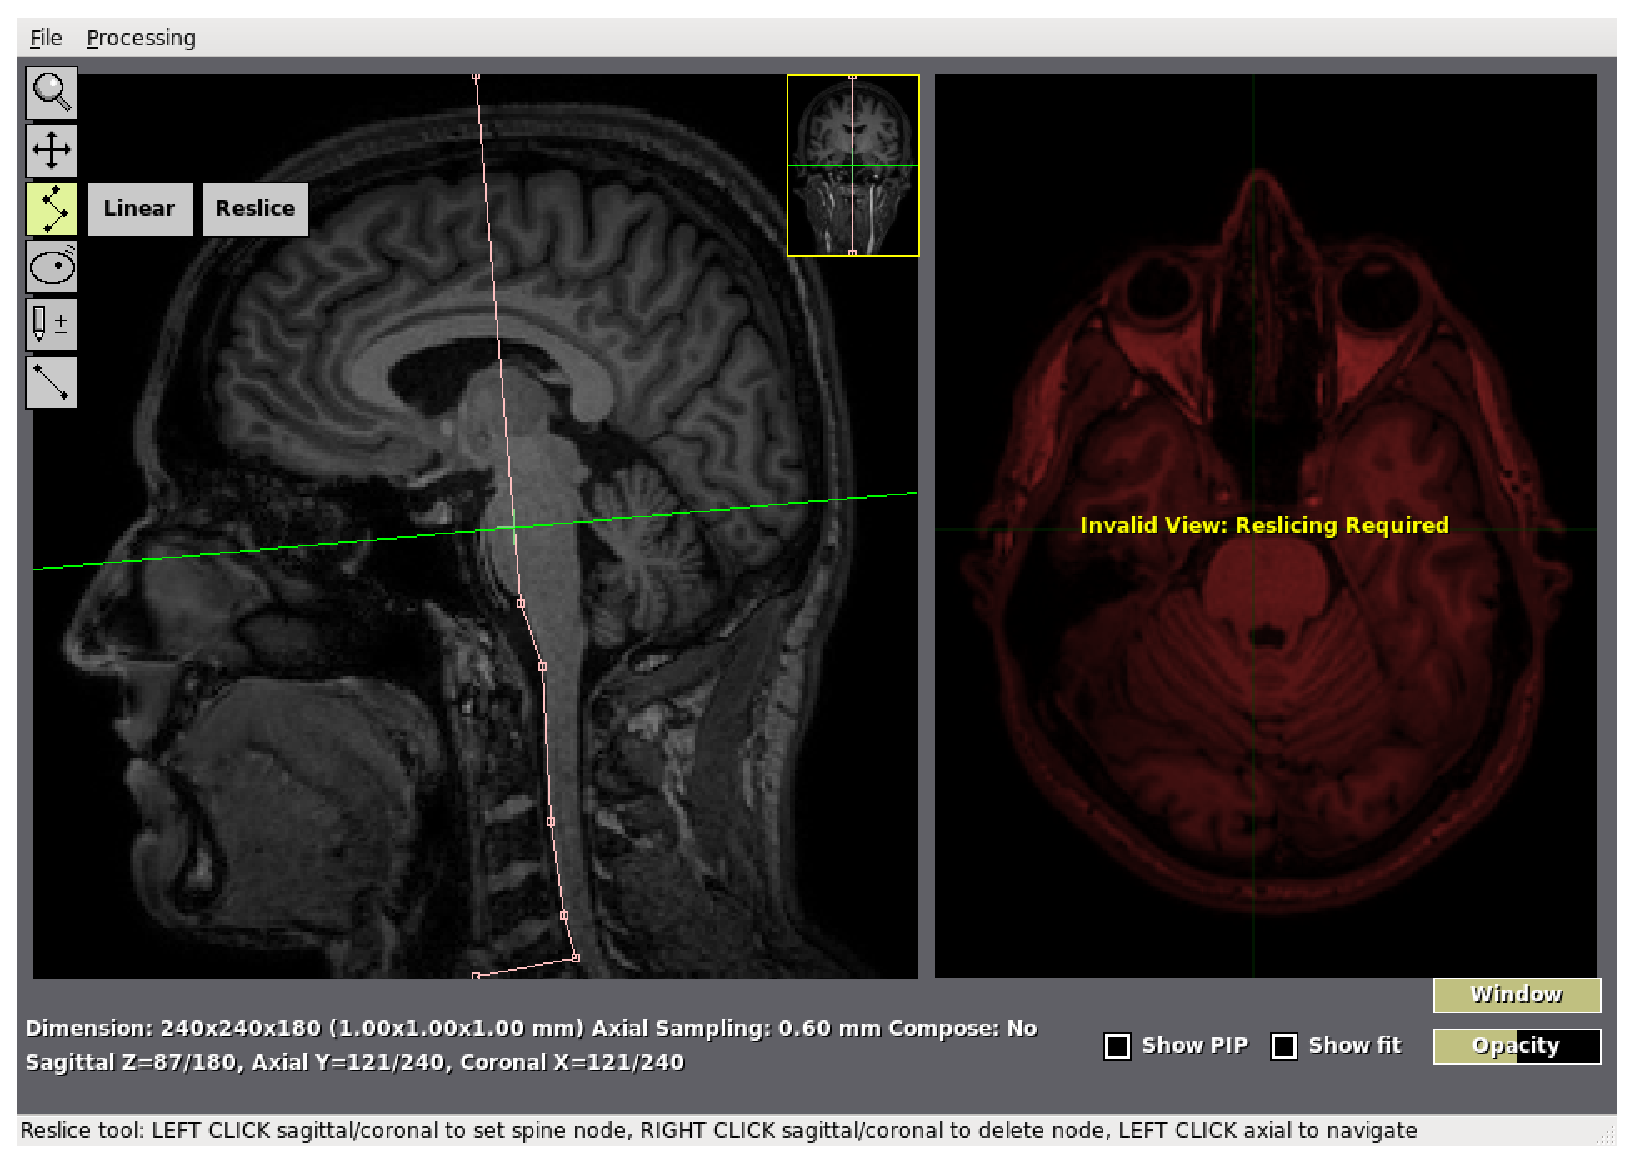
\includegraphics[width=12cm]{ex1.eps}
\caption{Sagittal reslicing guide.}
\label{f.ex1}
\vspace{20pt}
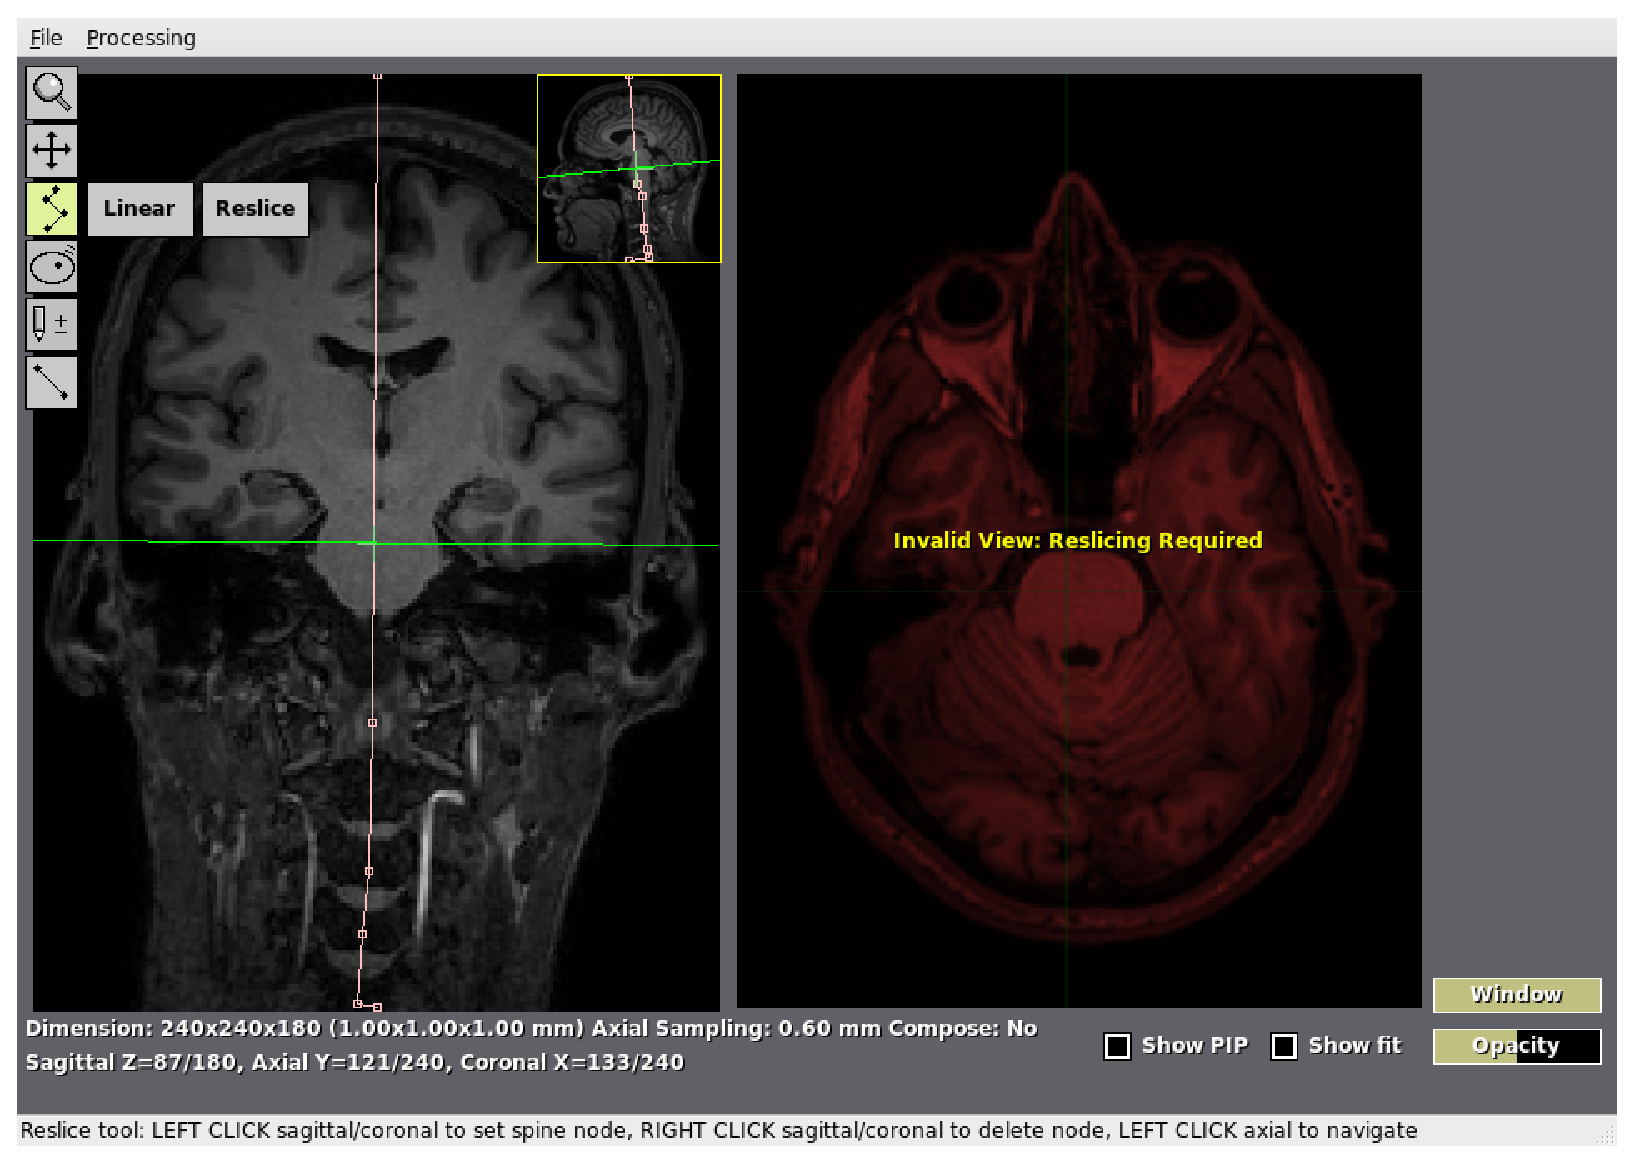
\includegraphics[width=12cm]{ex2.eps}
\caption{Coronal reslicing guide.}
\label{f.ex2}
\end{center}
\end{figure}


Clock on the \emph{Reslice} button and wait until reslicing is
complete. Select the semi-automatic segmentation tool. Click on the
PIP to switch back the left pane to sagittal slices. Use the up/down
keyboard arrow keys to locate a slice on the desired level for study.
In this example, we will measure the spinal cord at the top of the C3
vertebra, on the topomost slice where the disk between C2 and C3 no longer
appears. Press \texttt{Z} on the keyboard twice to select
4X axial zoom mode, and right click at the center of the spinal cord on the right
pane to segment it (Figure~\ref{f.ex3}).

\begin{figure}[!htb]
\begin{center}
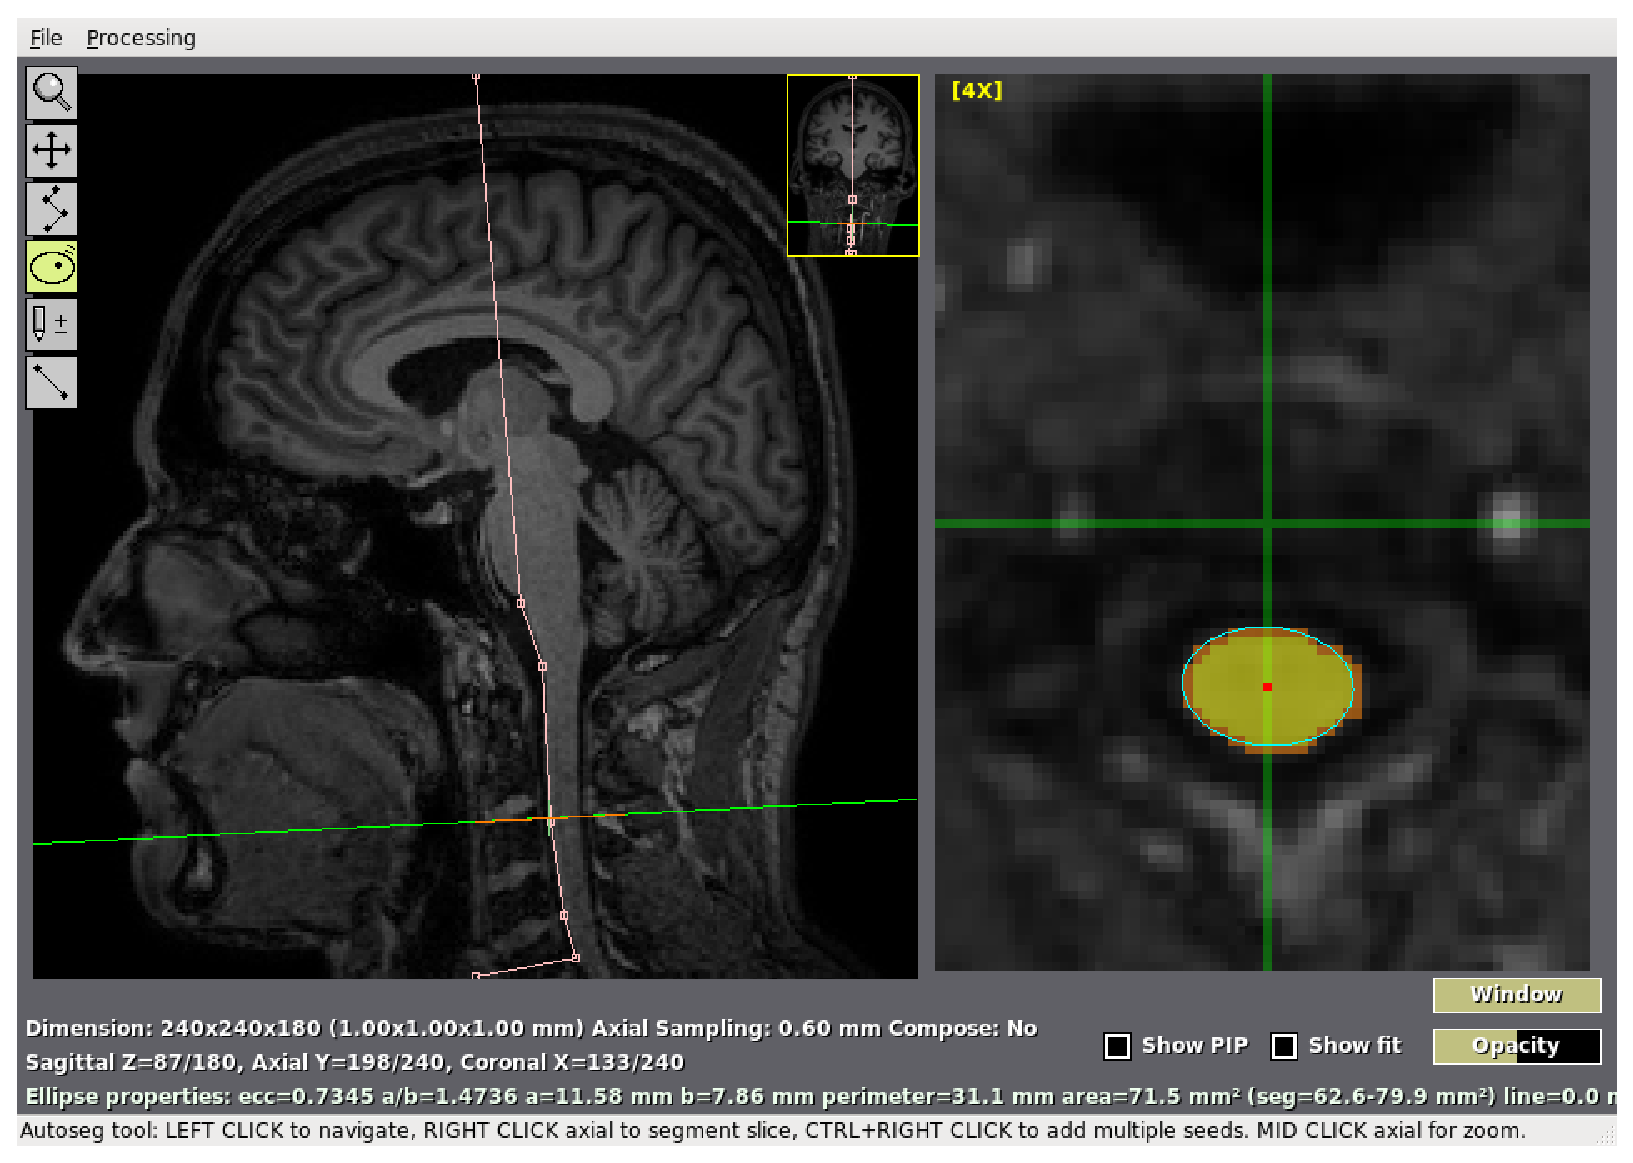
\includegraphics[width=12cm]{ex3.eps}
\caption{Spinal cord segmented.}
\label{f.ex3}
\end{center}
\end{figure}

If any distance measurement is desired, select the Distance measurement tool and left-click
both endpoints on the right pane. If you want to segment the spinal cord at other slices,
select the semi-automatic segmentation tool, navigate to the desired slice with the keyboard
arrow keys and repeat the procedure.

Once you are satisfied with the measurements, select \emph{File \btr Save State} to save
the results.

\chapter{Saved States}
\label{c.savestate}

When the current state is saved with the \emph{File \btr Save state}
command, SpineSeg splits state information into 8 files, written to
the same directory where the loaded volume file is located. The file
names are generated automatically based on the original file name. The
naming and format of each of these files is described below.

\section{Interpolated original volume}

When a volume without a saved state is first loaded by SpineSeg, it is
interpolated to make its resolution isometric, using the highest
resolution among the 3 axes.  E.g., a volume with voxel size $1.0
\times 1.0 \times 3.0$ mm is interpolated to $1.0 \times 1.0 \times
1.0$ mm.

When the state is saved, this interpolated volume is written to
\mybox{zzz\_BASENAME\_vol.scn} where \texttt{BASENAME} is the original
volume's filename stripped of the .scn extension, if it is present.
Despite the .scn extension, this file is saved compressed by
bzip2. This file is a 16-bit depth SCN file compressed with bzip2.

\section{Resliced volume}

The sequence of axial slices, interpolated to the enhanced axial
resolution and reformatted according to the guiding curves of the
reslice tool, is written to \mybox{zzz\_BASENAME\_rsd.scn} This
volume is also written as a 16-bit depth SCN file compressed with
bzip2.

\section{Segmentation volume}

A segmentation volume is written to \mybox{zzz\_BASENAME\_seg.scn}
This is an 8-bit label volume with the same dimension and resolution
of the resliced volume. Voxels with no segmentation are labeled with
0, internal voxels in segmented objects are labeled with 1, and border
voxels in segmented objects are labeled with 2.  This volume is
written as an 8-bit depth SCN file compressed with bzip2. Within
SpineSeg, the voxels labeled with 2 are the ones used to fit the
ellipses.

\section{Seeds volume}

A seeds volume is written to \mybox{zzz\_BASENAME\_see.scn} This is an
8-bit label volume with the same dimension and resolution of the
resliced volume. Seed voxels are labeled with 1, the remaining are
labeled with 0.This volume is written as an 8-bit depth SCN file
compressed with bzip2.

\section{Interface State}

The state of various interface controls is written to
\mybox{zzz\_BASENAME\_cfg.txt} This is a text file with 3 lines. The
first line contains 13 numeric values separated by spaces, lines 2 and
3 are comments. The values in the first line are, respectively:
current tool, cursor coordinate (Y), cursor coordinate (Z), overall
zoom level, pan coordinate (X), pan coordinate (Y), window saturation
level, opacity, show fit checkbox, show pip checkbox, cursor
coordinate (X), sagittal/coronal view state, stack composition state.

\section{Distance Measurement Locations}

The state of distance measurements is written to
\mybox{zzz\_BASENAME\_lin.txt} This is a text file with one measurement per
line. Each line has the form \texttt{y x1 z1 x2 z2}. Coordinates are given
in the domain of the resliced volume, and each line represents a line
segment $(x1,y,z1)-(x2,y,z2)$.

\section{Measurements}

The segmentation and distance measurement properties are written to
\mybox{zzz\_BASENAME\_fit.txt} This is a text file. The first line,
starting with \texttt{0file}, is a comment. The rest of the file is
one line for each slice with any measurements. Properties are comma-separated
and presented in this order: original volume file basename, Y coordinate of the slice, 
ellipse eccentricity, major/minor semi-axis ratio, major semi-axis (in mm), minor
semi-axis (in mm), ellipse perimeter in mm, ellipse area in mm$^2$, segmentation
area without the border (mm$^2$), segmentation area with the border (mm$^2$),
distance measurement length (mm). 

\section{Reslicing Curves}

The reslicing guiding curves are written to
\mybox{zzz\_BASENAME\_rsv.txt} This is a text file with one line per
control point. Sagittal control points are in the form \texttt{x X Y},
where $(X,Y)$ is the coordinate of the control point, and coronal
control points are in the form \texttt{z Z Y}, where $(Z,Y)$ is the
coordinate of the control point. A line with the word \texttt{spline}
indicates spline interpolation mode for the reslicing guides. Absence
of this line indicates linear mode.



\end{document}

